\documentclass[a4paper]{article}

\usepackage{fullpage}
\usepackage{graphicx}
\usepackage{subcaption}
\usepackage{url}
\usepackage{hyperref}
\usepackage{acronym}
\usepackage{paralist}
\usepackage{amsmath}
\usepackage{lipsum}
\usepackage{booktabs}
\usepackage{float}
\usepackage{listings}
\usepackage[official]{eurosym}
\usepackage[ruled,vlined]{algorithm2e}


% ----------------------------------------------------------------------------
% Start the document
%
\begin{document}


\begin{centering}
~~~~~~~~~~~~~\\[-20mm]

  {
  \bfseries Master Degree in Computer Science\\[3mm]
  Web Architectures\\[3mm]
  AA 2014-2015
  }\\[1mm]


  \vspace{0.5cm}
  {
  \Large \bfseries{Java Enterprise Application} \par
  }
  {
  \small \bfseries{Project report} \par
  }
  \vspace{0.2cm}

  {Davide Spadini (id 164393)}

  \vspace{0.3cm}
\end{centering}



\section{Introduction}
\label{sec:intro}
With this project I want to implement a \emph{Java Enterprise Application} that simulates the website of a Bank, enabling the user to log in and check its account, create a transaction to another client, withdraw or refill money from its account.

The application is divided in 3 parts:
\begin{compactitem}
  \item \textbf{Web Tier} Containing all the JSF pages and the Managed Beans
  \item \textbf{Business Tier} Containing the entity class, two stateless beans and one stateful bean
  \item \textbf{Persistent Tier} Database that contains all the users
\end{compactitem}

\noindent
The Web Tier runs on Tomcat, the last two on Wildfly instead.

\section{Settings and Usage}
\label{sec:settings}
In order to work the project needs:
\begin{compactitem}
  \item Tomcat: download at \url{http://tomcat.apache.org/download-80.cgi}
  \item Wildfly: downloat at \url{http://wildfly.org/downloads/}
  \item DerbyDS: download at \url{https://db.apache.org/derby/derby_downloads.html}
\end{compactitem}

\noindent
I created a directory that is available at \url{TODO} in which there are all the necessary configurations and there is already the project inside. In this case, you can jump to Section~\ref{subsec:start}, otherwise in the next sections we will see how to setting up from scretch the environment.
\subsection{Setting up Tomcat}
\label{subsec:tomcat}
Tomcat starts by default on the port 8080, widlfy too. So we need to modify the file 

\verb|TOMCAT_HOME/conf/server.xml|

\noindent
changing the line 69 from ``port=8080'' to ``port=9090''. Then we copy the file \verb|BankDSWeb.war| in the directory \verb|TOMCAT_HOME/webapps|.

\subsection{Setting up Wildfly}
\label{subsec:wildfly}
In order to work with DerbyDS, we have to add in the file

\verb|WILDFLY_HOME/standalone/configuration/standalone.xml|

\noindent
the following code inside the tag \verb|<datasources>|:

\begin{verbatim}
  <datasource jndi-name="java:/DerbyDS" pool-name="DerbyDS" enabled="true" use-ccm="false">
      <connection-url>jdbc:derby://localhost:1527/JbossDB;create=true</connection-url>
      <driver-class>org.apache.derby.jdbc.ClientDriver</driver-class>
      <driver>derbyclient.jar</driver>
      <security>
          <user-name>demo</user-name>
          <password>demo</password>
      </security>
      <validation>
          <validate-on-match>false</validate-on-match>
          <background-validation>false</background-validation>
      </validation>
      <statement>
          <share-prepared-statements>false</share-prepared-statements>
      </statement>
  </datasource>
\end{verbatim}

\noindent
Then we have to copy the file 

\verb|DERBY_HOME/lib/derbyclient.jar|

\noindent
to:

\verb|WILDFLY_HOME/standalone/deployments/|

Finally, we copy the file \verb|BankDS.ear| to \verb|WILDFLY_HOME/standalone/deployments|.

\subsection{Start the project}
\label{subsec:start}
First of all, we need to start DerbyDS, so in the terminal:

\begin{verbatim}
  export DERBY_HOME=YOUR/PATH/TO/db-derby-10.11.1.1-bin
  $DERBY_HOME/bin/setEmbeddedCP
  mkdir $DERBY_HOME/databases
  pushd $DERBY_HOME/databases/
  java -jar $DERBY_HOME/lib/derbyrun.jar server start &
  popd
\end{verbatim}

Then we start Wildfly:
\begin{verbatim}
  ./WILDFLY_HOME/bin/standalone.sh
\end{verbatim}

Finally start Tomcat:
\begin{verbatim}
  ./TOMCAT_HOME/bin/startup.sh
\end{verbatim}

Now the administrar page is available at \verb|http://localhost:9090/BankDSWeb/admin.xhtml| in which you can add a new user, then with the username and password inserted you can login in 

\noindent
\verb|http://localhost:9090/BankDSWeb/login.xhtml|.


\section{Use Case}
\label{sec:req_analysis}
The application can be used by an ``administrator'' or a ``user'': the first one can add or delete a new user and he has the complete list of them; the second one has associated a checking account and a credit card, he can make a bank transaction to another client, he can withdraw/refill money from/to its checking account or credit card. The complete Use Case Diagram is shown in Figure~\ref{fig:use_case_diagram}.

\begin{figure}[ht]
  \centering
  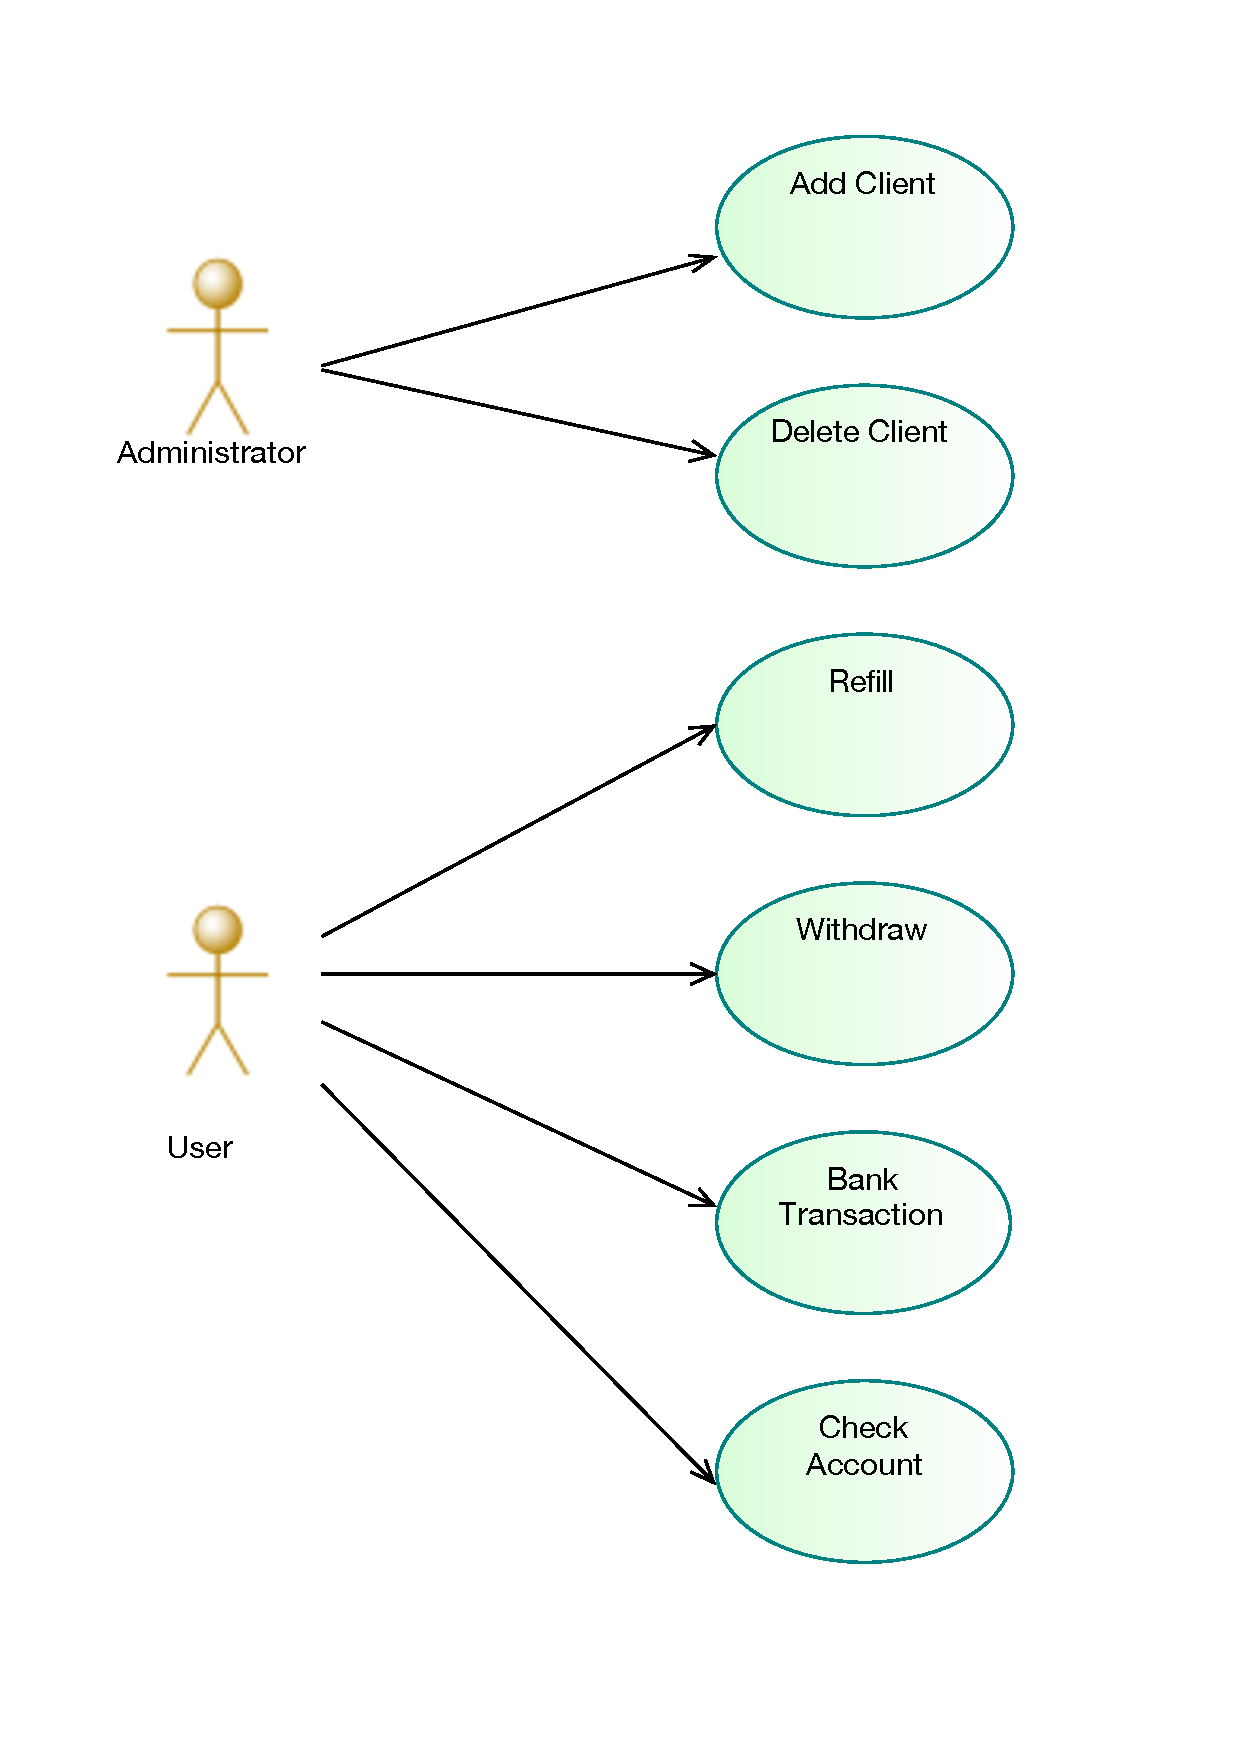
\includegraphics[keepaspectratio=true, width=5cm]{use_case_diagram}\caption{Use case Diagram.}
  \label{fig:use_case_diagram}
\end{figure}

\section{Design}
\label{sec:design}
The project is divided in 3 main parts: the web tier, the business logical tier, the persistent tier. In Figure~\ref{fig:classdiagram} there is the complete Class Diagram, and in the next subsections we will see briefly what is the content of each layer.

\subsection{Web Tier}
\label{subsec:webtier}
This tier is divided in 2 categories: the web pages and the java class. For the first one I use JSF pages with a template; for the second one I use two Managed Beans and one java class that allow me to connect remotely to the business tier. The beans are explained in details in Section~\ref{sec:impl_details}.

\subsection{Business Logical Tier}
\label{subsec:bus_log_tier}
In this tier we can found the EJB beans and the interface that the web tier uses to call remotely the business methods. The EJB module, as shown in Figure~\ref{fig:classdiagram}, contains three beans (two stateless and one stateful) and one entity: the user. Furthermore, I don't represented in the class diagram, there are other two classes that represents the exceptions.

\subsection{Persistent Tier}
\label{subsec:pers_tier}
I use Apache Derby\footnote{More information at url \url{https://db.apache.org/derby/}} as database: I created just one table that represents the list of users and their informations. In Section~\ref{sec:impl_details} we will see how the beans can access to the database.

\begin{figure}[ht]
  \centering
  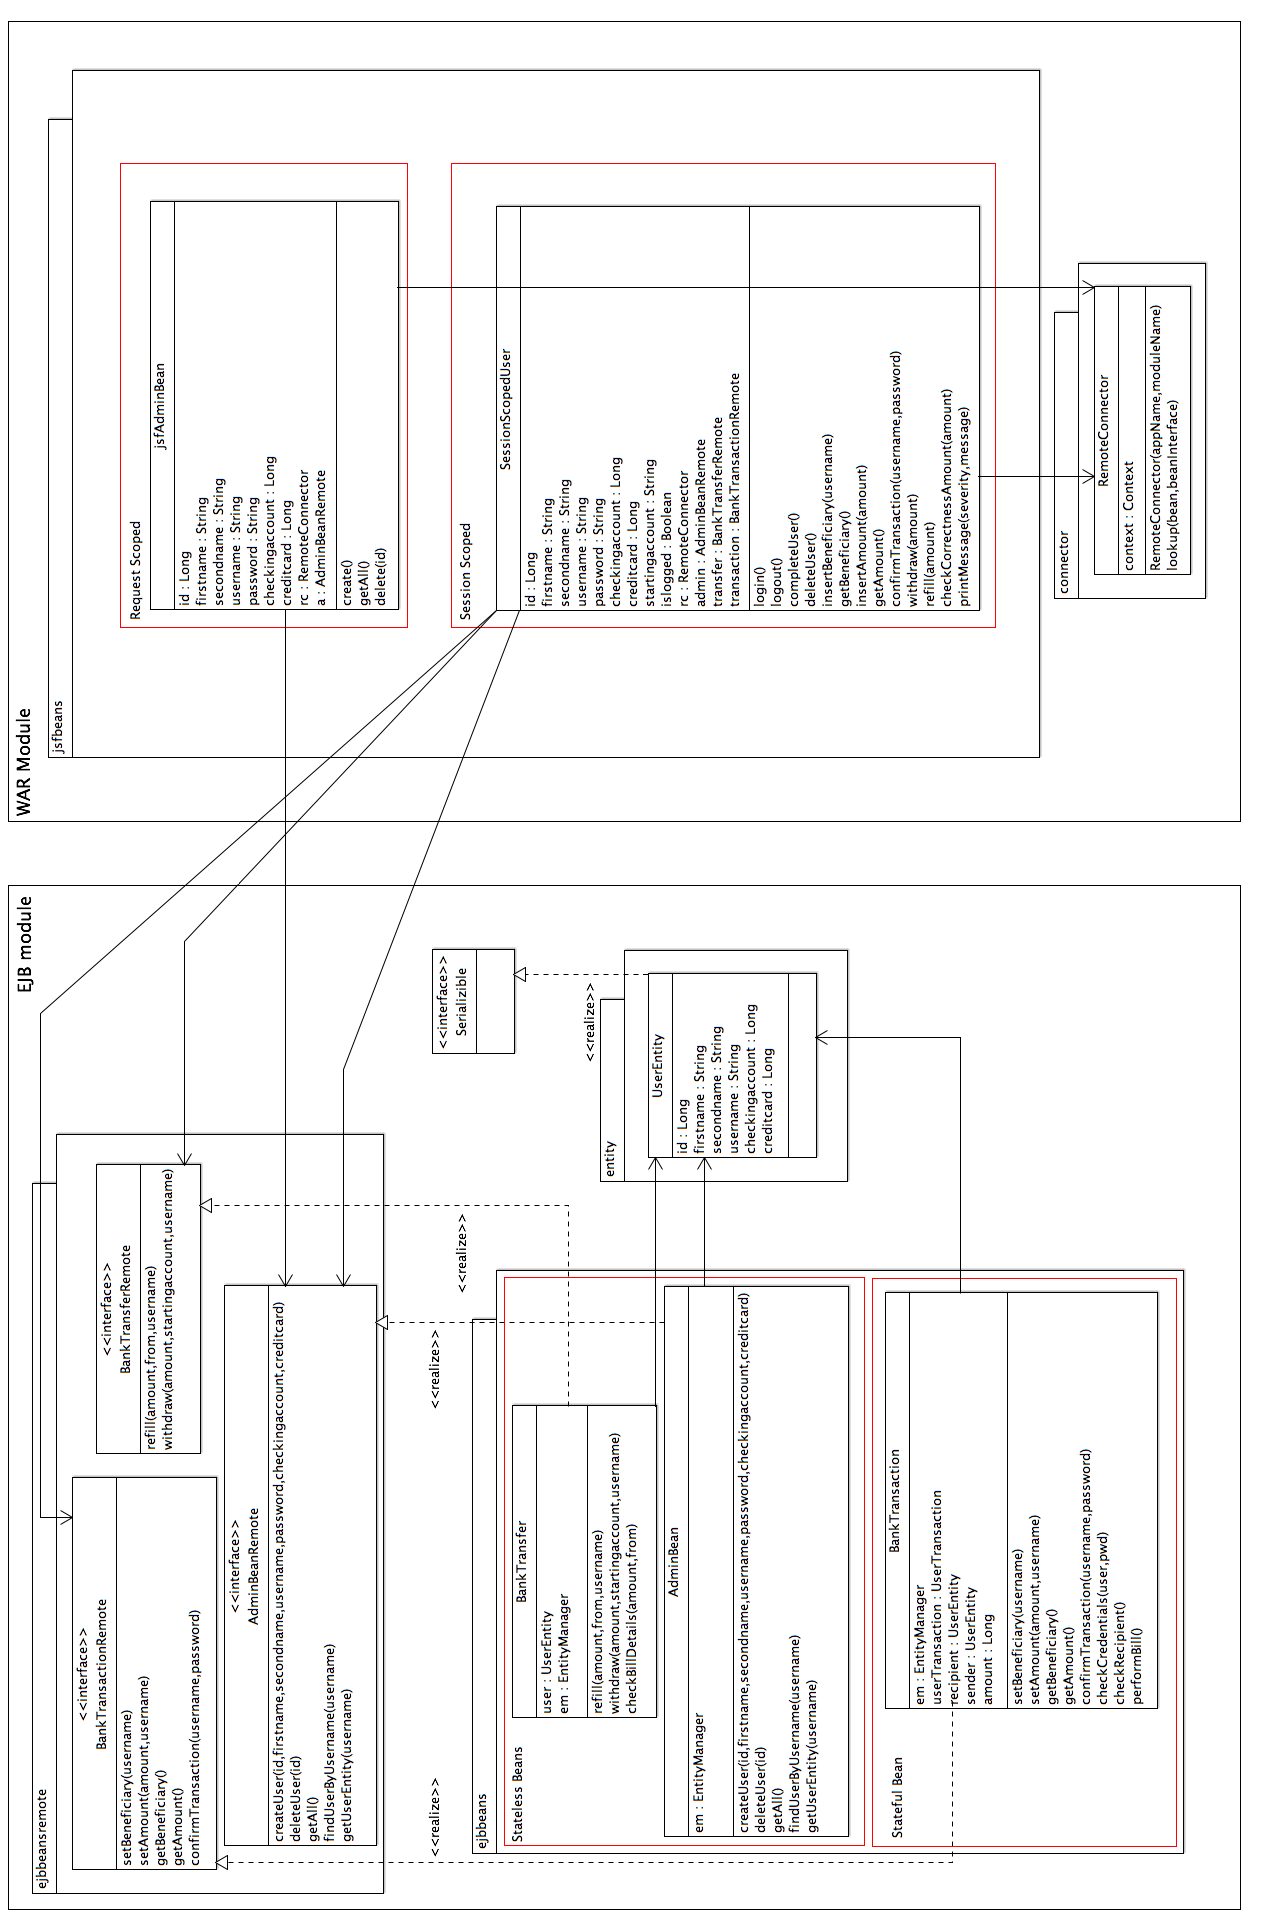
\includegraphics[keepaspectratio=true, width=\textwidth, height=\textheight]{ClassDiagram2.png}\caption{Use case Diagram.}
  \label{fig:classdiagram}
\end{figure}

\section{Implementation Details}
\label{sec:impl_details}
In this section I will explain in detail the various technologies that I used and how I implemented the various tiers. 

\subsection{EJB Beans}
\label{subsec:ejb}
In the project there are three beans:
\begin{compactitem}
  \item \textbf{AdminBean} this is a stateless bean. It has five functions that can be called remotely: createUser, deleteUser, getAll (returns a list of users), findUserByUsername, getUserEntity (returns all the informations about a user).
  \item \textbf{BankTransfer} this is a stateless bean. It has just two functions that can be called remotely: refill and withdraw. Furthermore it has minor functions that checks if the informations inserted by the user are correctly (i.e. if he has enough money to withdraw, etc etc). 
  \item \textbf{BankTransaction} this is a stateful bean. Indeed, when a user wants to create a transaction, it has to passed through three steps: insert the beneficiary, insert the amount, confirm the transaction. This three steps are executed in different pages, so in order to remember the previous choices of the user I use a stateful bean. There are five functions that can be called remotely: setBeneficiary, get Beneficiary, setAmount, getAmount, confirmTransaction. The most important is the last one: in fact in this function I use a transaction. The reason why I do that is explained in Section~\ref{subsec:trans}. There exists other minor functions that are not called remotely that checks the correctness of the payment.
\end{compactitem}

All the beans are equipped with a ``EntityManager'' in order to save the results of the operations in the database. The EntityManager interface defines the methods that are used to interact with the persistence context.

\subsection{JSF Beans}
This beans serve the requests of the user (through JSF page) calling remotely the appropriate EJB beans. The package ``jsfbeans'' contains two Managed Beans:
\begin{compactitem}
  \item \textbf{jsfAdminBean} its duty is to complete the JSF page of the administrator with the data collected calling the functions of the ``AdminBean'', and allow the administrator to create or delete a user. It has ``request scope''.
  \item \textbf{SessionScopedUser} differently from the previous bean it has ``session scope'' (see Section~\ref{subsec:login}). It is the most important one: in fact it has to serve the requests of the user from the moment that he logs in until he logs out.
  When a user enters in the website, this bean obtains the necessary informations about him from the ``AdminBean'', then when a user wants to create a transaction it calls the ``BankTransaction'' bean or when he wants to withdraw it calls the ``BankTransfer'' , the same for the refill.
\end{compactitem}

\subsection{RemoteConnector}
\label{subsec:rem_conn}
As I said before the Application Server runs on Wildfly, while the Web Application on Tomcat. So in order to work:
\begin{enumerate}
  \item EJBs have to be accessible remotely from the JSF beans, so the annotation ``@Remote'' is used
  \item the JSF Managed Beans has to invoke EJBs via JNDI: the java class ``RemoteConnector'' is used.
\end{enumerate}

When a JSF bean is initialized and it wants to obtain a reference to the remote object, it calls the function ``lookup'' of this class passing the name of the bean and the name of the interface of the bean that it needs. Once is called, the lookup method sets the necessary properties and return a proxy that the JSF bean will use to communicate with the server\footnote{Given that I use Wildfly 8, I used the ``jboss-remote-naming''\cite{remotejndi}}.

\subsection{Transaction}
\label{subsec:trans}
When a user creates a bank transaction, he has to insert the beneficiary, insert the amount and then confirm the transaction inserting his username and password. In each step the correctness of the information inserted by the user are checked, but since it can takes longer from the moment he began to the end, the account informations can change. We can consider this situation: I have \euro{1000} on my account and I want to transfer all this money to a friend, so I set the beneficiary, I set the amount to \euro{1000} (the system checks if I have enough money and it let me pass to the next step), then I don't confirm and I wait here. In the meanwhile, I open another tab and I withdraw all the money from my account, then I return on my transaction and I click confirm. The transaction should goes wrong because I don't have enough money, it succeeded instead. This because from the moment that the system checks the amount of money of the transaction, my account has changed (in particular, I withdraw all the money). So in order to handle this situation, I inserted a ``TransactionManagement'' in the code of the relative bean. When a user click confirm, a new transaction is created and it checks:
\begin{itemize}
  \item if the beneficiary still exists
  \item if the bill details are correct (i.e. enough money)
  \item if the username and password inserted are correctly
\end{itemize}

If one of this three checks fail, all the transaction fails and an error is shown. In the other case, the transaction succeed.

\subsection{Log In}
\label{subsec:login}
All the JSF pages load a template and they fulfill the necessary informations. In this template I use the tag ``ui:fragment'' to check a flag in the SessionScoped Bean that is true if the user is logged in, false otherwise. I use this tag as ``if else'' in Java:

\verb|<ui:fragment rendered="#{sessionScopedUser.islogged}">|
\verb|</ui:fragment>|

\noindent
If ``islogged'' is true, then all the content inside the tag is shown, otherwise it is not. 
Then when a user logs out the flag is set to false, and all the JSF pages will redirect the user to the log in page.

\subsection{CSS Template}
\label{subsec:css}
In order to have a better representation and a more user-friendly website I used a modified version of the CSS available at \url{http://ironsummitmedia.github.io/startbootstrap-business-casual/}. The graphics of the website is partially shown in Figure~\ref{fig:gui1} and Figure~\ref{fig:gui2}.


\begin{figure}[h]
  \begin{subfigure}{0.5\textwidth}
    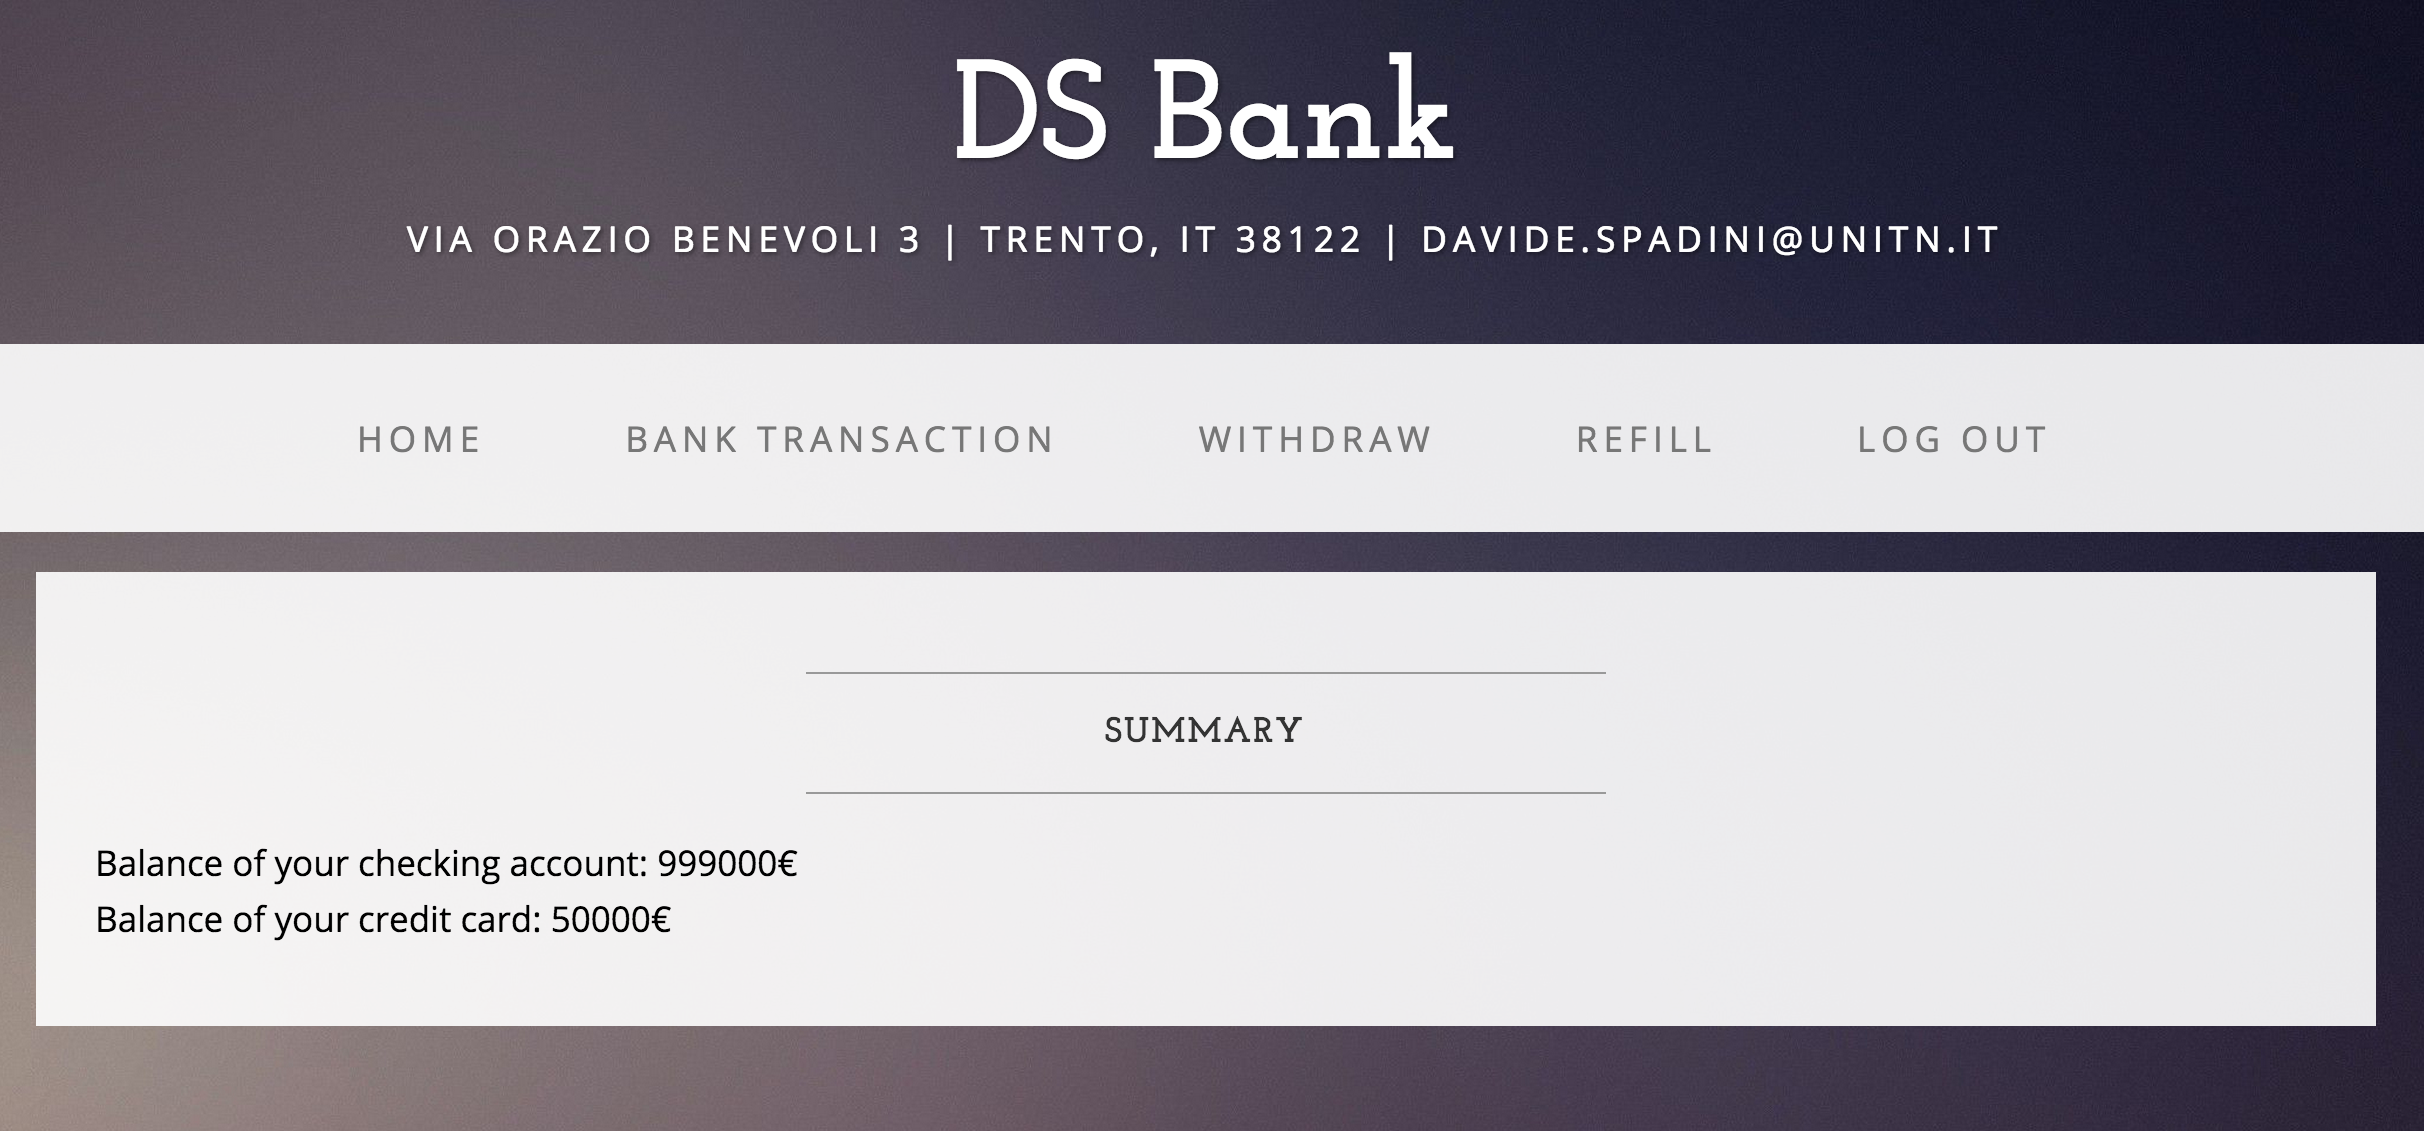
\includegraphics[keepaspectratio=true, width=0.9\linewidth, height=10cm]{home}
    \caption{Home}
    \label{fig:home}
  \end{subfigure}
  \begin{subfigure}{0.5\textwidth}
    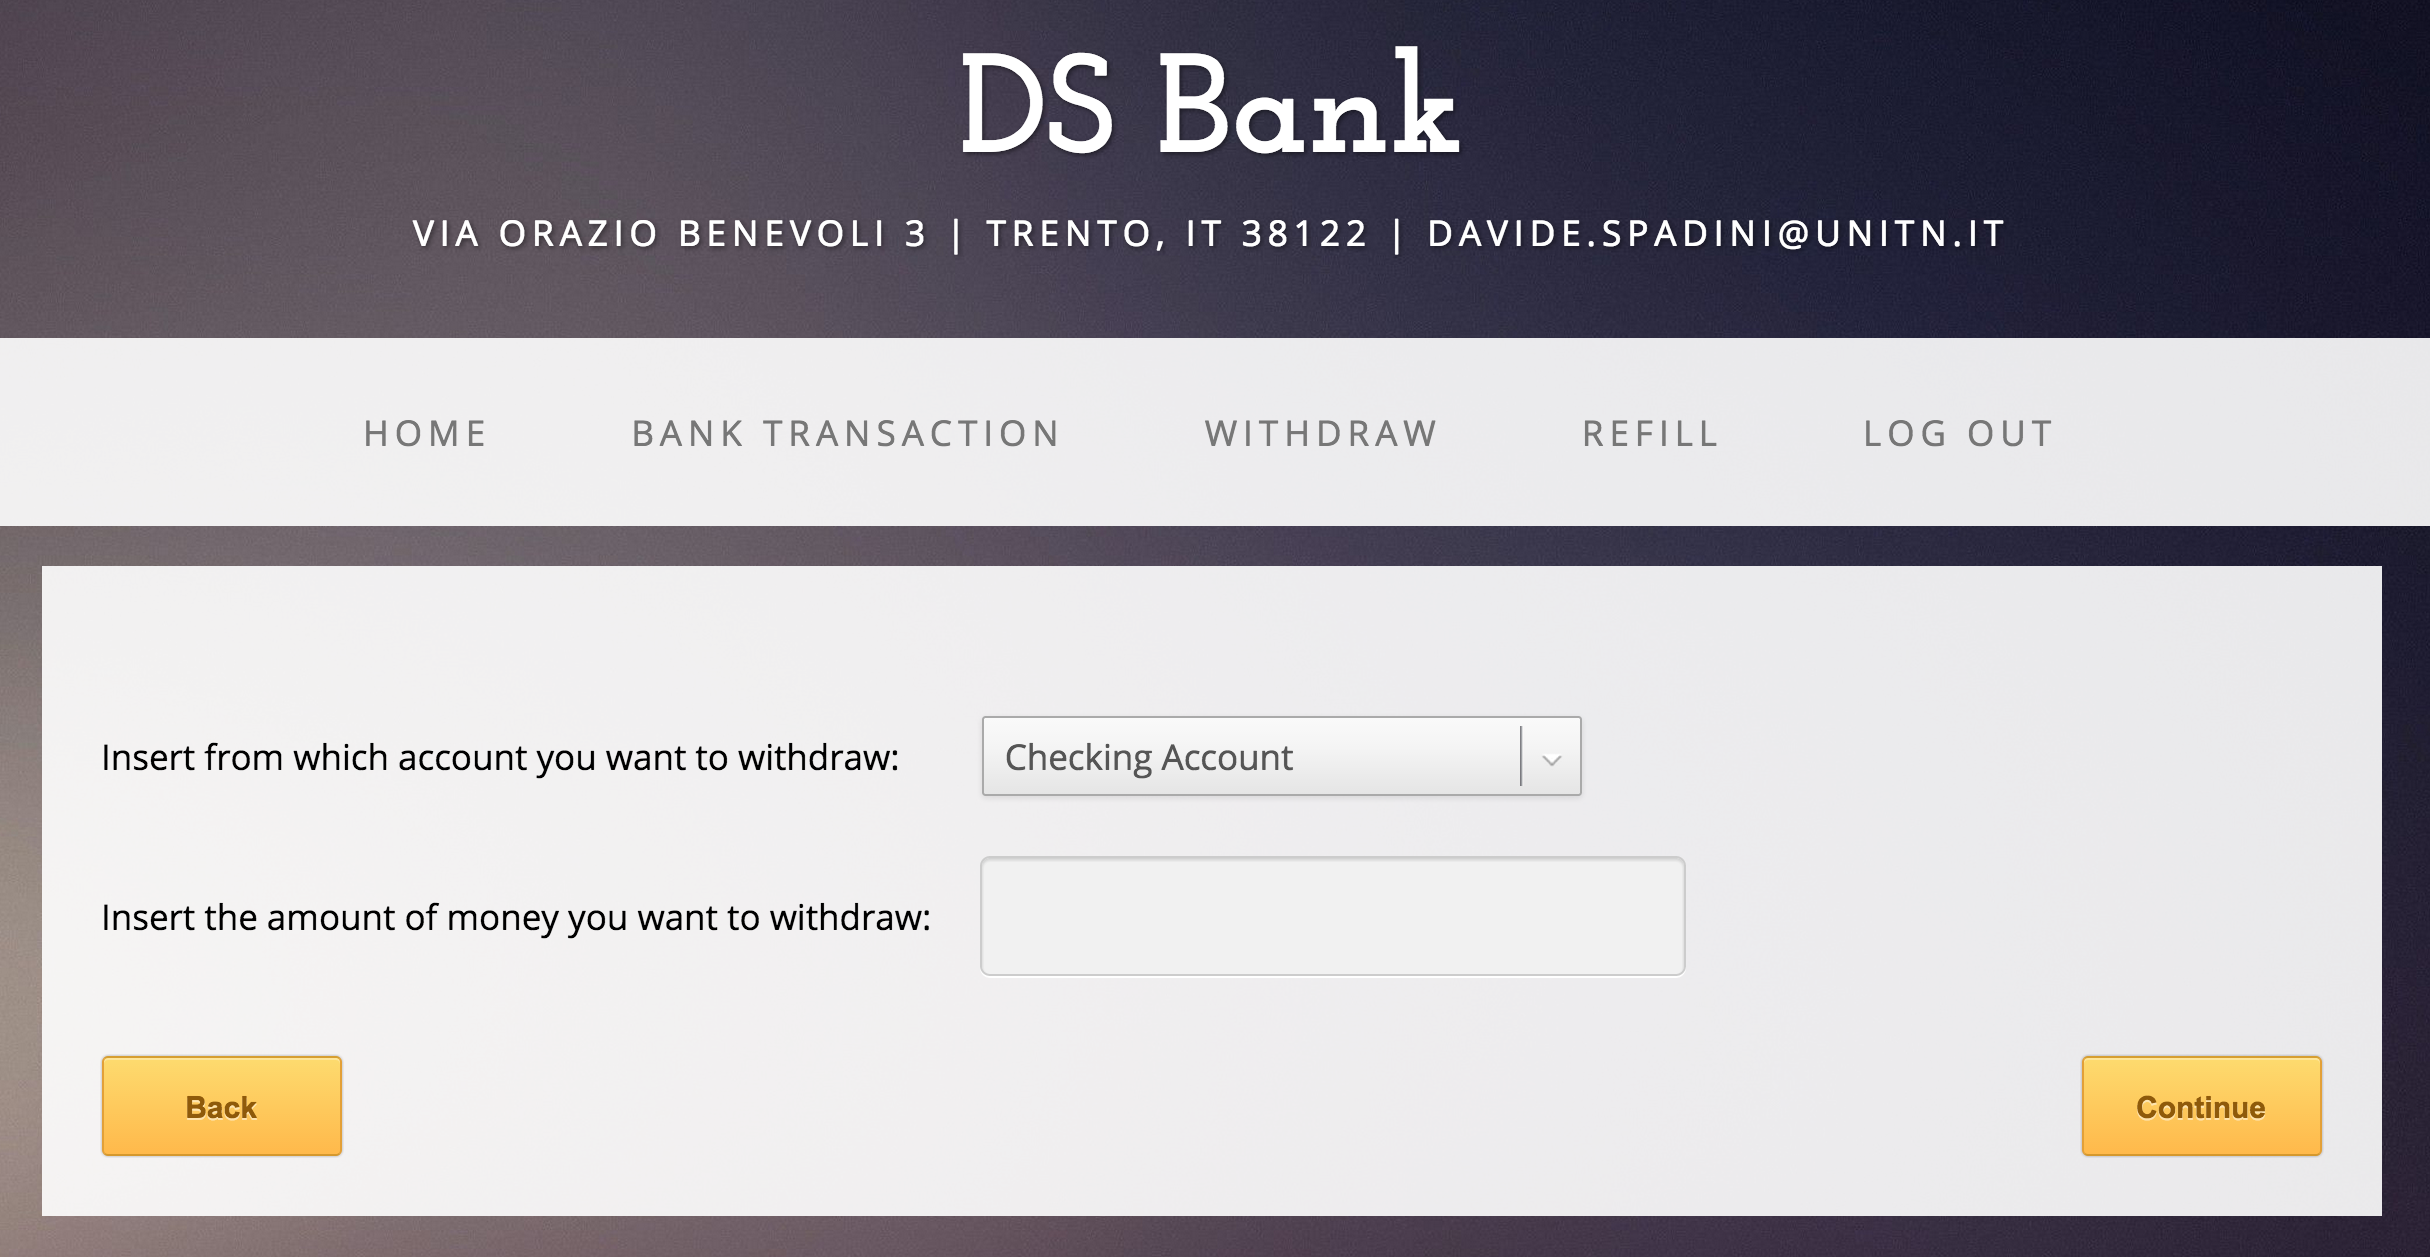
\includegraphics[keepaspectratio=true, width=0.9\linewidth, height=10cm]{refill} 
    \caption{Refill}
    \label{fig:refill}
  \end{subfigure}
  \caption{Graphic of the Home page and Refill page}
  \label{fig:gui1}
\end{figure}

\begin{figure}[h]
  \begin{subfigure}{0.5\textwidth}
    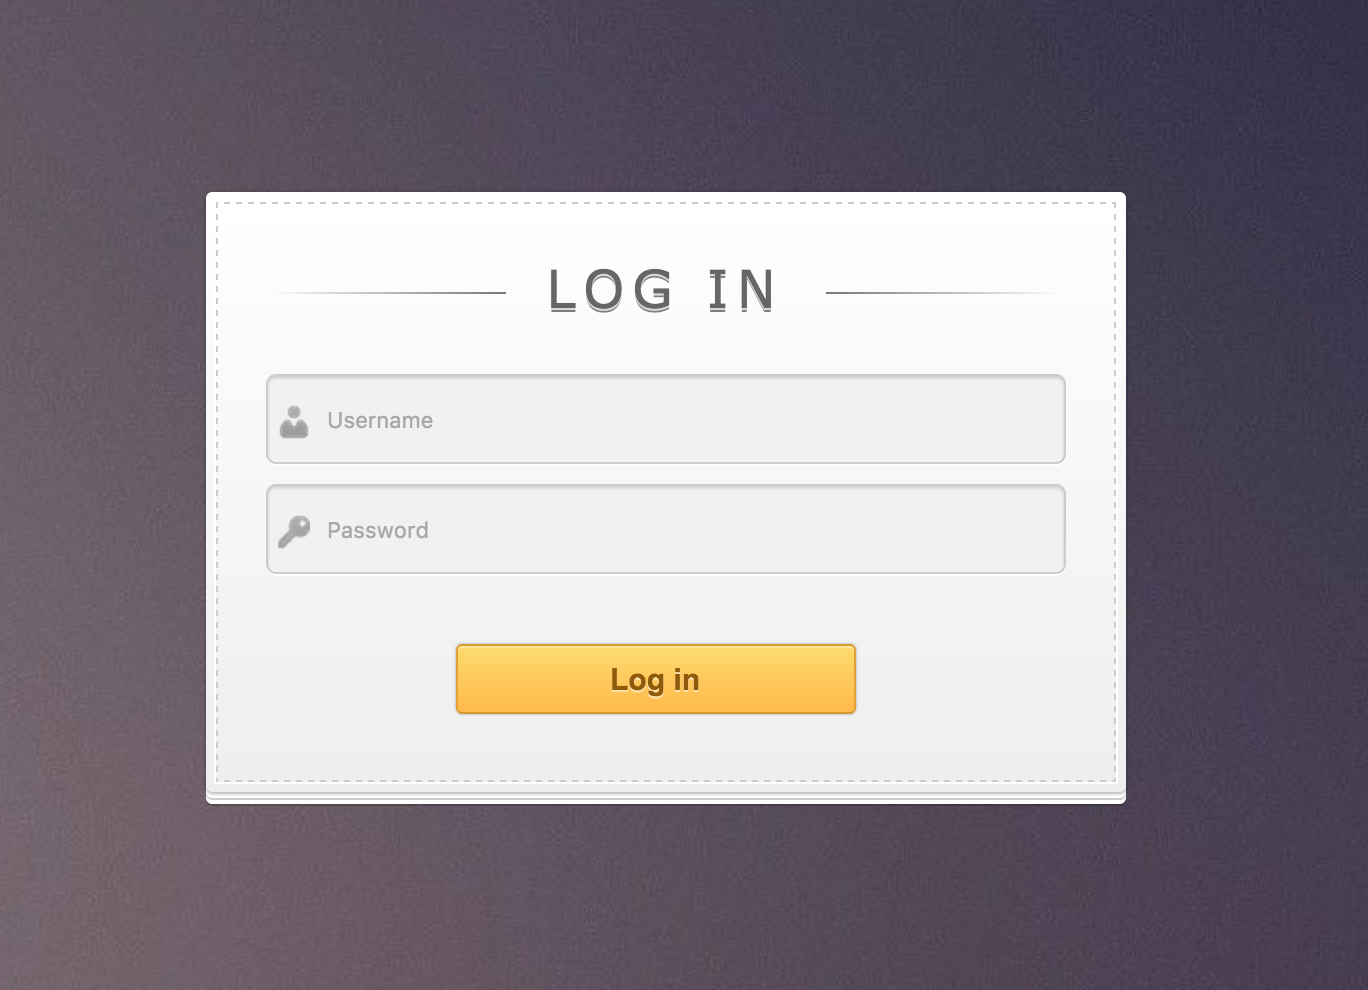
\includegraphics[keepaspectratio=true, width=0.9\linewidth, height=10cm]{login}
    \caption{Login}
    \label{fig:login}
  \end{subfigure}
  \begin{subfigure}{0.5\textwidth}
    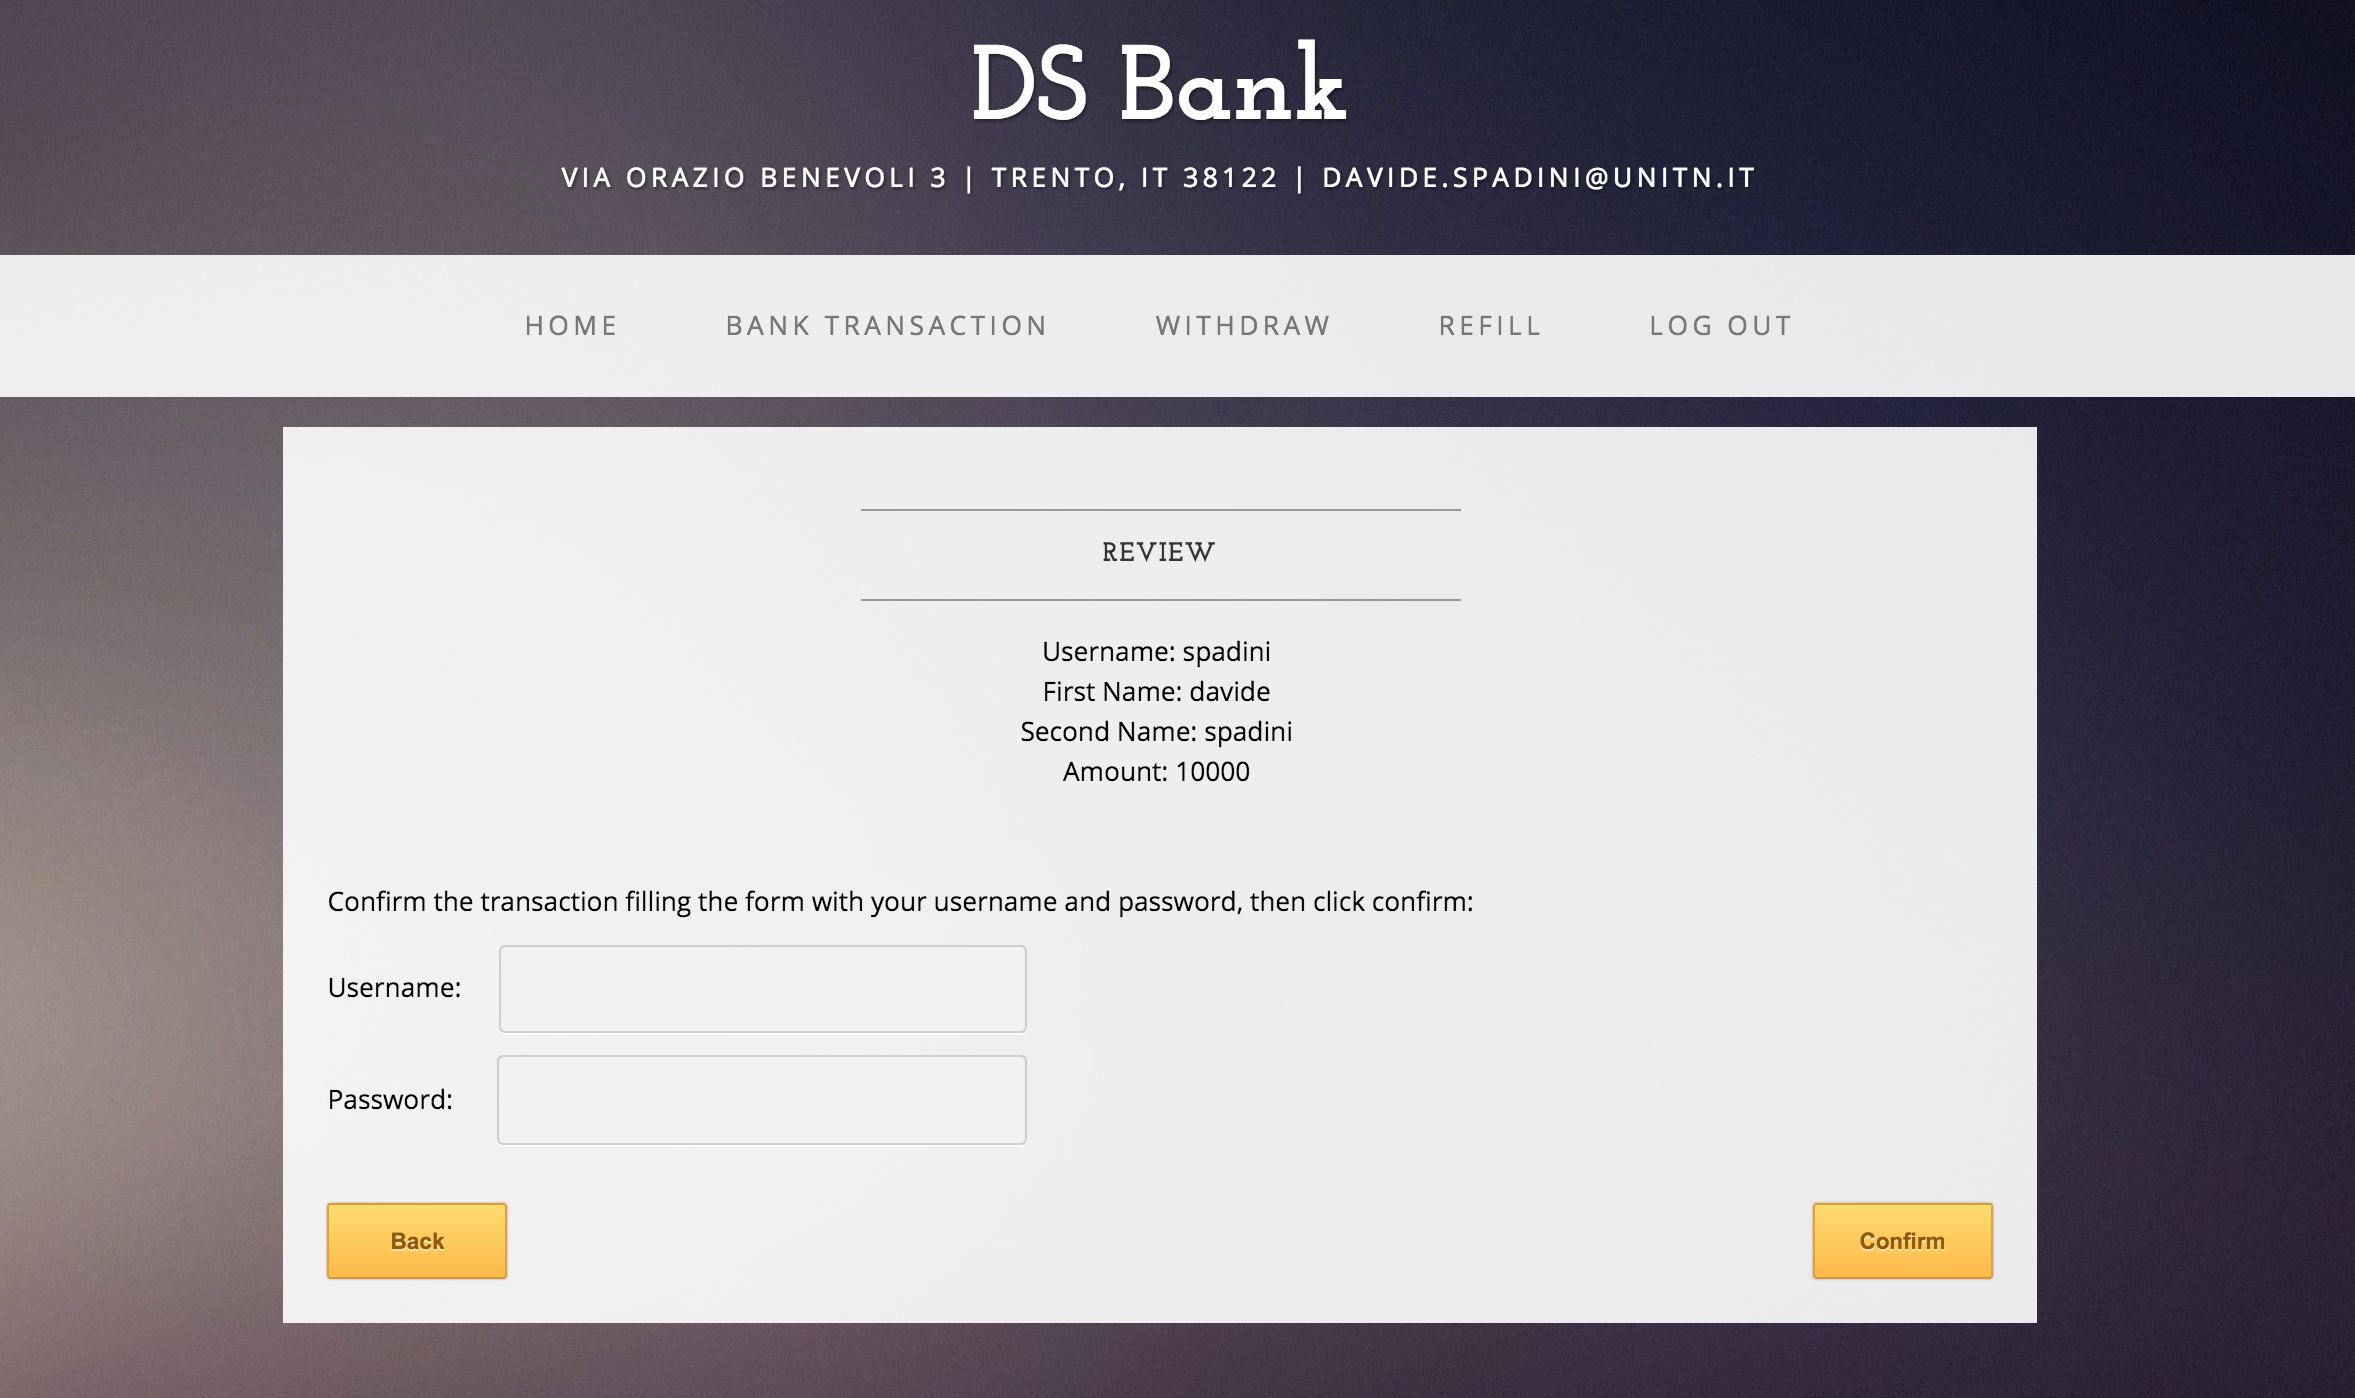
\includegraphics[keepaspectratio=true, width=0.9\linewidth, height=10cm]{transaction} 
    \caption{Transaction}
    \label{fig:transaction}
  \end{subfigure}
  \caption{Graphic of the Login page and Transaction page}
  \label{fig:gui2}
\end{figure}


\section{Comments and Notes}
\label{sec:conc}
For the entire duration of the project I kept a blog in which I wrote the encountered problems, how I solved them and what I should do next: the blog is available at \url{webarchitectures.davidespadini.it}. However, a possible recap of the major problems is:
\begin{compactitem}
  \item \textbf{set the environment} I found very difficult set correctly Wildfly, Tomcat, Netbeans and DerbyDS to work together correctly
  \item \textbf{Separating the Web and Business Tier} initially, my project ran on Wildfly. When I finished it I tried to split the Web Server from the Application Server, using Tomcat and Wildfly. Here the problem was that the Web Application that I wrote didn't work on Tomcat (problem with the last version of JSF), so I had to re-created it in Netbeans including the Tomcat server. Furthermore, I had to insert the remote interfaces and change all the functions in the EJBs that return or accept as parameters an entity.
\end{compactitem}
\noindent


\bibliographystyle{plain}

\begin{thebibliography}{5}

\bibitem{models} Montresor A.
\textit{Models}. Retrieved 15:39, May 11, 2015, from
\url{http://disi.unitn.it/~montreso/ds/handouts/02-models.pdf}


\bibitem{fdconsensus} Montresor A.
\textit{Consensus with failure detectors}. Retrieved 15:39, May 11, 2015, from
\url{http://disi.unitn.it/~montreso/ds/handouts/07-fdconsensus.pdf}

\bibitem{remotejndi}
\textit{Remote EJB invocations via JNDI - EJB client API or remote-naming project}
\url{https://docs.jboss.org/author/display/WFLY8/Remote+EJB+invocations+via+JNDI+-+EJB+client+API+or+remote-naming+project}

\end{thebibliography}

\end{document}
